% Skrivet av Nils

Primtal är förrädiskt oförutsägbara.
De dyker upp när du minst anar det och kan till synes bete sig totalt oregelbundet.
Trots detta är de helt deterministiska i sin natur och gränsen för vad som är och inte är ett primtal är mycket tydlig.
Det är kanske just av denna anledning som primtalen, även i modern tid, är så intressanta att studera.


Hur många primtal finns det? Svaret är att det finns oändligt många.
Om vi istället frågar oss hur många primtal det finns som är mindre än en miljon, så är svaret inte lika lätt.
Till att börja med vet vi att primtal, med undantag för talet 2, aldrig är jämna.
Därför kan vi åtminstone utesluta vartannat tal och säga att svaret är mindre än en halv miljon.
Hur går vi vidare härifrån?
Ett naturligt andra steg vore att föra samma resonemang för talet 3;
förutom just 3 så är primtal aldrig delbara med 3 och därmed borde vi kunna dra bort ytterligare en tredjedels miljon från svaret.
Detta är dessvärre inte riktigt sant.
Tal som både är jämna och delbara med 3 har ju uteslutits två gånger.
Det har alltså skett en dubbelräkning av alla tal som kan delas med 6,
men vi kan kompensera för detta genom att addera en sjättedels miljon till svaret.


Denna uppskattning av svaret är bättre än den vi hade tidigare och givetvis kan vi fortsätta vidare med talet 5.
På så sätt skulle vi komma ännu närmre det faktiska svaret, 
men vi skulle också behöva hantera fler dubbelräkningar.
Den generella idén här kallas för \textit{inklusions-exklusionsprincipen} och illustreras nedan för tre mängder med hjälp av figur \ref{pop.fig}.

\begin{figure}[H]
    \centering
    % Skrivet av Nils

\usetikzlibrary{shapes,backgrounds}

\def\rad{1.5}
\def\dcircle{.95}
\def\dinnertext{1}
\def\doutertext{1.5}



\def\angA{330}
\def\angB{90}
\def\angC{210}

\def\circleA{(\angA:\dcircle) circle [radius=\rad]}
\def\circleB{(\angB:\dcircle) circle [radius=\rad]}
\def\circleC{(\angC:\dcircle) circle [radius=\rad]}

\vspace{0.2cm}
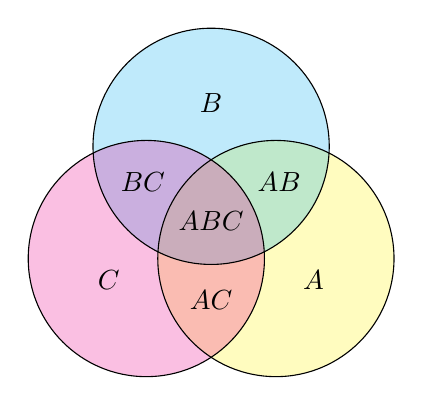
\begin{tikzpicture}
    \begin{scope}[fill opacity=0.25]

        \fill[yellow] \circleA;
        \fill[cyan] \circleB;
        \fill[magenta] \circleC;
        \draw \circleA;
        \draw \circleB;
        \draw \circleC;
    \end{scope}
    \node at (\angA:\doutertext) {$A$};
    \node at (\angB:\doutertext) {$B$};
    \node at (\angC:\doutertext) {$C$};
    \node at ({(\angA+\angB-360)/2}:\dinnertext) {$AB$};
    \node at ({(\angB+\angC)/2}:\dinnertext) {$BC$};
    \node at ({(\angA+\angC)/2}:\dinnertext) {$AC$};
    \node at (0,0) {$ABC$};
\end{tikzpicture}
    \caption{Illustration av inklusions-exklusionsprincipen för tre stycken överlappande mängder $A$, $B$ och $C$.}
    \label{pop.fig}
\end{figure}

\begin{comment}
\begin{figure}[H]
    \centering
    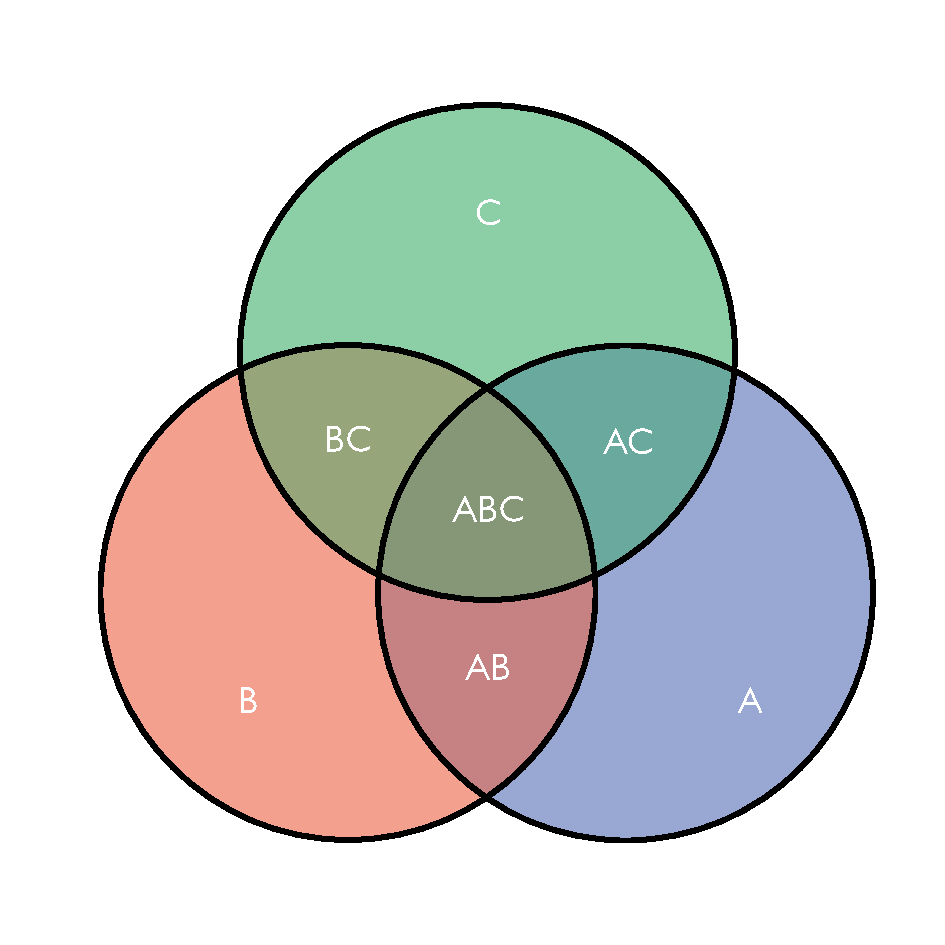
\includegraphics[scale=0.3]{erik/Images/Venndiagram.pdf}
    \caption{Illustration av inklusions-exklusionsprincipen för tre stycken överlappande mängder $A$, $B$ och $C$.}
    \label{pop.fig}
\end{figure}
\end{comment}

Säg att vi vill beräkna den totala storleken för de överlappande mängderna $A$, $B$ och $C$. 
Vi kan börja med att summera storleken på mängderna var för sig.
Om vi betecknar storleken på $A$ som $|A|$ och gör på samma vis för de andra mängderna så kan vi skriva summan som $|A|+|B|+|C|$.
Som bekant har det skett en dubbelräkning där mängderna överlappar varandra.
Låt oss skriva $AB$ när vi menar överlappet mellan $A$ och $B$, och liknande för de andra överlappen.
Precis som i tidigare exempel kompenserar vi för dubbelräkningen genom att dra bort dessa överlapp ifrån summan, vilket ger oss $|A|+|B|+|C|-|AB|-|BC|-|AC|$.
%$AB$, $BC$ samt $AC$, vi drar bort dessa från summan och får $|A|+|B|+|C|-|AB|-|BC|-|AC|$.
Vidare har vi även $ABC$ där alla tre mängderna överlappar varandra.
Denna ingår i alla tidigare nämnda mängder och har därmed lagts till och dragits bort tre gånger om. 
Vi lägger till $ABC$ en gång till och kommer fram till det slutgiltiga svaret
\begin{equation*}
    |A|+|B|+|C|-|AB|-|BC|-|AC|+|ABC|.
\end{equation*}
Detta är inklusions-exklusionsprincipen och den kan användas för ett godtyckligt antal mängder.
Metoden att använda denna princip för att räkna primtal kallas för \textit{Legendres såll} och är fundamental i teorin om matematiska såll.


Ett (matematiskt) såll är i stora drag en metod för att rensa bort vissa tal ur en mängd heltal.
Som ovan exempelvis, då vi använde Legendres såll för att sålla bort icke-primtal ur mängden av heltal upp till en miljon.
I denna rapport presenteras tre stycken såll;
\textit{Eratosthenes generaliserade såll}, \textit{Bruns såll} samt \textit{Selbergs såll} som alla bygger på idéer liknande det vi har sett här.
Gemensamt för de tre sållen är att de inte ger något exakt svar, eftersom ett sådant ofta är opraktiskt att jobba med.
Istället nöjer vi oss med approximationer, vilket ändå kan vara användbart förutsatt att vi känner till storleken på uppskattningens fel.
Dessa feltermer och deras beteende utgör en väsentlig skillnad mellan de olika sållen och en diskussion samt jämförelse av feltermerna är således relevant. Därför har detta tillägnats en egen del i rapporten vilken följer efter att de tre sållen presenterats.


I rapportens sista avsnitt redogör vi för hur Harald Helfgott i \cite{HaraldSieve} har utvecklat idéer från ett grundläggande såll för att skapa effektiva algoritmer som kan utföras med en dator. 
Därefter framlägger vi vår implementation av algoritmerna i ett program skrivet i Python.
Avslutningsvis presenteras även några resultat som vi fått från att köra programmet,
där ett av resultaten knyter an till frågan om att räkna primtal.
Men istället för att som ovan, titta på tal mellan noll och en miljon, har vi valt att svara på frågan för ett intervall med mittpunkt i $10^{19}$ och en bredd på $2.5\times10^9$.